\section{Previous Work}

    Previous researchers have worked to understand and replicate the phenomena described in Section \ref{Natural Systems} in the laboratory environment. They have laid the groundwork for the current project by investigating the fields of vortex sensing with lateral lines and tandem foil wake interaction. To the knowledge of the current team, no previous work has ever applied lateral line technology to a tandem fin control system, and this possibility would link the work of previous researchers to more effective control systems.

\subsection{2D Wake Interaction} \label{2D Wake Interaction}

    Although fish fins are flexible and three dimensional, simplifying their interactions by considering 2D rigid systems composed of their cross sections has allowed for experimental analysis of their wake interactions. Three coherent modes of wake interaction have been observed between flapping foils: constructive, destructive, and vortex pairing \citep{Gopalkrishnan1994}. When foils are phase shifted such that like-rotating vortices meet at the trailing edge of the downstream foil, the vortices build constructively into a single, larger vortex. The two foils create one vortex street with increased circulation. When foils are phase shifted such that oppositely rotating vortices meet, the vortices combine destructively, resulting in dramatically decreased circulation. The resultant vortex street is of the same shape as the vortex street for a single foil, but with reduced circulation. When the foils are not in such a phase that would cause one of the wakes above, the shed vortices meet and pair downstream of both foils and create a double street wider than the street from a single foil \citep{Gopalkrishnan1994}.

\subsubsection{Effects of 2D Wake Interaction} \label{Effects of 2D Wake Interaction}

    Due to the complex fluid dynamics equations governing the wake interactions between flapping foils, the effects of wake interaction have been largely studied through experimental means \citep{Boschitsch2014}. The wake interaction directly impacts the thrust and power coefficients on the trailing foil, with the largest coefficients associated with constructive vortex interactions and the lowest coefficients associated with destructive interactions \citep{Gopalkrishnan1994, Boschitsch2014, Muscutt2017}. Additionally, the foil spacing also influences the vortex interaction. When the spacing between two foils is greater than one half of their chord length, the wake interaction has negligible impact on the dynamics of the upstream foil \citep{Boschitsch2014}.

\subsubsection{Parameters Governing 2D Wake Interaction} \label{Parameters Governing 2D Wake Interaction}

    The degree of wake interaction is dependent on the phase difference between the foils, the Strouhal number, and the foil spacing \citep{Boschitsch2014, Muscutt2017}. These parameters dictate the mode of wake interaction between the foils, as well as the strength of their impact on the coefficients of thrust and power on the downstream foil, which can be observed in \Fref{fig:PW:Thrust vs Phase}. This figure compares the coefficients of thrust, \(C_T\), and power, \(C_P\), for a single fin with those of a downstream fin in a tandem configuration. As the lighter regions indicate, various combinations of phase difference, $\phi$, between tandem fins and the fins' spacing, \(\frac{s}{C}\), cause large improvements in downstream foil performance, e. g. $C_T^*$ at $\frac{s}{C}=1.5$ and $\phi=\frac{7\pi}{4}$. \citep{Boschitsch2014} used foils that only made pitching motions to create \Fref{fig:PW:Thrust vs Phase}, but similar results also occur for foils that pitch and heave \citep{Gopalkrishnan1994, Muscutt2017}.

\begin{figure}
\begin{center}
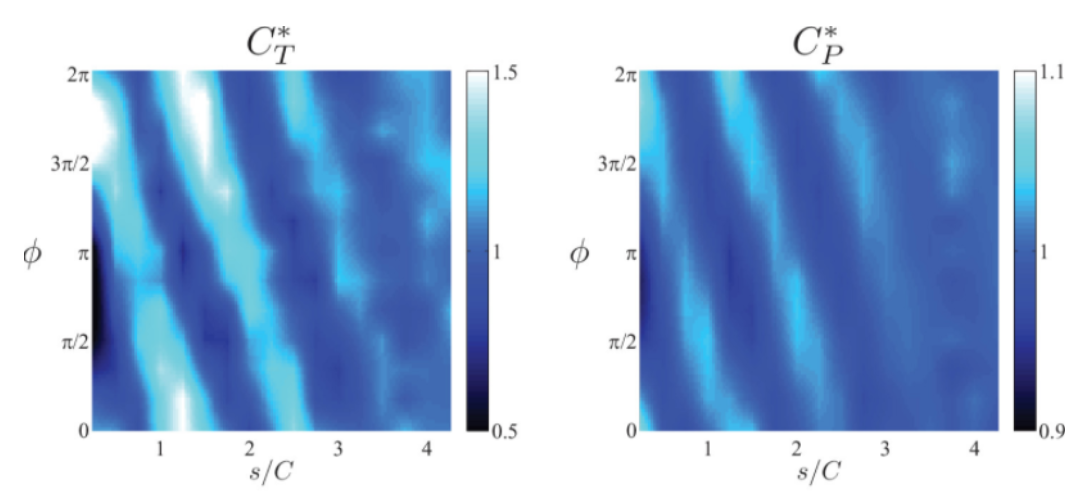
\includegraphics[width=0.8\columnwidth]{figures/Bos Results.png}
\end{center}
\caption{Variation of normalized thrust coefficient (left) and power coefficient (right) on a downstream foil with respect to phase difference in radians, \(\phi\), and foil spacing in units of foil chord lengths, \(s/C\). The coefficients are normalized by dividing by the coefficients experienced by a single flapping foil under the same parameters, as \(C_T^*=\frac{C_{single foil}}{C_{tandem foil}}\). Lighter regions indicate parameter combinations that offered improved characteristics relative to a single flapping foil, and darker regions indicate combinations that decreased characteristics \citep{Boschitsch2014}.}
\label{fig:PW:Thrust vs Phase}
\end{figure}

% Cam 12/29: talk about specific numbers of thrust improvement? Take a paragraph to explain why it's valuable to control the wake interaction? Should this paragraph be placed later in the proposal?

\subsection{Human Made Lateral Lines} \label{Human Made Lateral Lines}
 
    Several groups have developed artificial canal neuromasts using microelectromechanical systems (MEMS) \citep{Fan2002, Chen2007, Kottapalli2014} , or optical sensors \citep{Klein2011}. However, because CNs detect pressure differences across the surface of fish, many researchers have implemented off-the-shelf pressure sensors to achieve similar effects \citep{Venturelli2012} \citep{DeVries2015} \citep{Zhang2015}. These configurations eliminate the need for a canal, as the differential pressure between two points can be calculated by simply subtracting the measurements from adjacent sensors. The lateral lines become linear arrangements of sensors, such as the arrays built by \citep{Venturelli2012} and \citep{Fernandez2011}, shown in \Fref{fig:PW:Human Lateral Lines}. The sensors are embedded in a structure and make contact with the water through holes in the surface.

\begin{figure}
\begin{center}
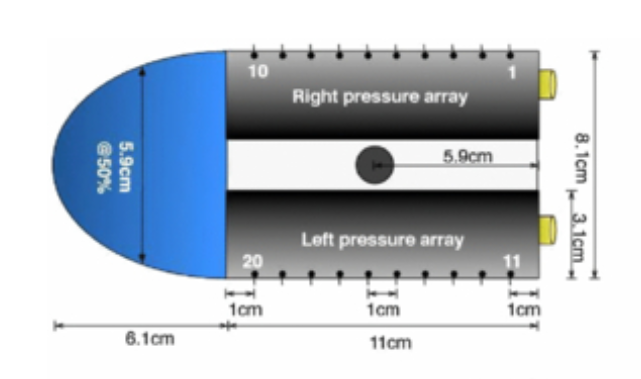
\includegraphics[width=0.60\columnwidth]{figures/Venturelli Setup.png}
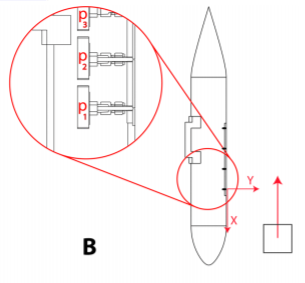
\includegraphics[width=0.30\columnwidth]{figures/Fernandez Setup.png}
\end{center}
\caption{Linear pressure sensor array designed to detect oncoming vortices using absolute pressures, where each black dot represents an MS5401-BM pressure sensor (left) \citep{Venturelli2012}. Linear array of Honeywell 19C015PG4K pressure sensors used for classifying nearby objects (right) \citep{Fernandez2011}.}
\label{fig:PW:Human Lateral Lines}
\end{figure}

\subsection{Vortex Wake Feature Extraction with Lateral Lines} \label{Vortex Wake Feature Extraction with Lateral Lines}

    Pressure sensor arrays have demonstrated the ability to draw both qualitative and quantitative characteristics from object wakes. As described in Section \ref{Karman Vortex Streets}, vortices produce low pressure regions in the water. These vortex streets create perceptible undulations in the readings from differential pressure sensor arrays, as can be seen in \Fref{fig:PW:Venturelli Results}. This pressure data was generated by \citep{Venturelli2012} when they placed the array shown in \Fref{fig:PW:Human Lateral Lines}(left) behind a cylinder in steady flow. The vortices, represented by the alternating bands of red and blue, have both a time and magnitude associated with them. The time measured between vortices allows for calculation of the oscillation frequency, while the time one vortex takes to reach a sensor of a known distance away allows for calculation of the flow speed. In \Fref{fig:PW:Venturelli Results}, this is visible in the diagonal shape of the red and blue bands, as the vortices are measured by each sensor as they are advected downstream by the underlying uniform flow. Downstream sensors detect vortices later than upstream units. The flapping frequency observed by the sensors is apparent at any perpendicular displacement from the vortex street, as seen in \Fref{fig:PW:Chambers Results}, although the signal to noise ratio decreases as the sensor array makes less contact with the vortices \citep{Chambers2014}. \Fref{fig:PW:Chambers Results} also shows that the frequency perceived by a sensing array is constant when its movement within the street is small, as moments where frequencies peaked occurred at moments when the array was moving fastest \citep{Chambers2014}.  In the case of flapping foils, the vortex shedding frequency, \(f_h\), and free stream flow speed, \(U_\infty\), are two of the three terms related to the Strouhal number, according to \ref{Eq:Fin St}. This Strouhal number corresponds directly to the efficiency, thrust, and power of the foil. As shown by these studies, linear pressure sensor arrays have the potential to indicate the effective Strouhal number of a system and, thus, offer real-time feedback on the performance of a system. 
    
    While the artificial lateral line response to a single Karman vortex wake is well documented, no studies to date have characterized its response in the presence of two interacting vortex wakes. This research project will perform experiments to understand how these sensors would perceive such a wake.
% how to say that the frequency reading is robust as long as the sensor array is still?
\begin{figure}
\begin{center}
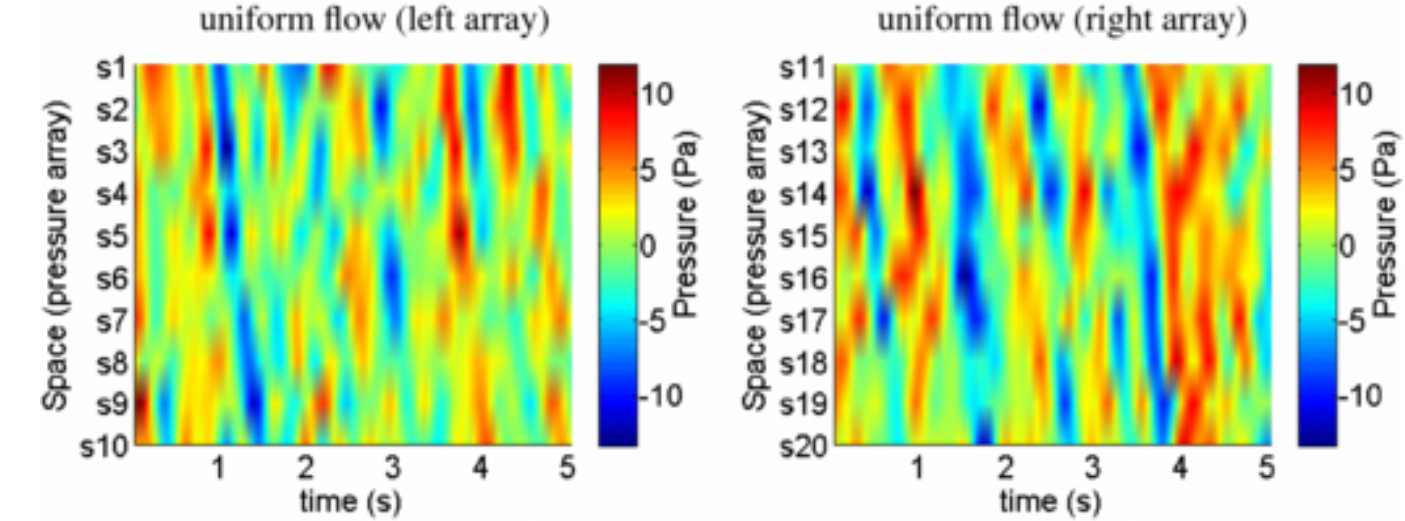
\includegraphics[width=0.80\columnwidth]{figures/Venturelli Readings.PNG}
\end{center}
\caption{Pressure readings from each sensor on the artificial lateral line shown in \Fref{fig:PW:Human Lateral Lines}(left). Higher numbered sensors on the same plot are farther downstream than the lower numbered sensors. Pressure readings are encoded by color and correspond to the vortices shed by an upstream cylinder \citep{Venturelli2012}.}
\label{fig:PW:Venturelli Results}
\end{figure}
\begin{figure}
\begin{center}
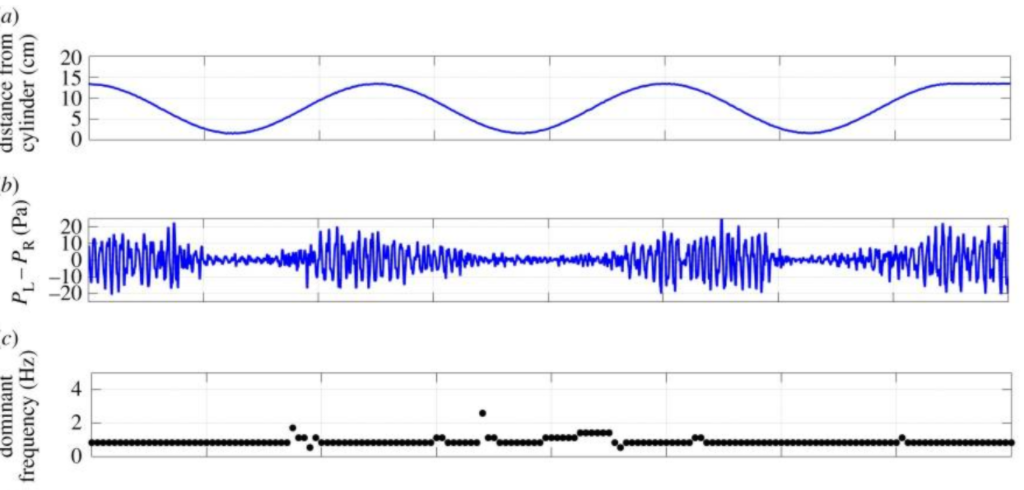
\includegraphics[width=0.80\columnwidth]{figures/Chambers Lateral Results.PNG}
\end{center}
\caption{A pressure sensing array's lateral displacement from a Karman vortex street with respect to time (top). Differential pressure readings between the left and right sides of an array as it moved into and out of the vortex street (middle). The dominant frequency observed at each moment in the array's path (bottom) \citep{Chambers2014}.}
\label{fig:PW:Chambers Results}
\end{figure}

    Lateral line-inspired systems consisting of commercially available pressure sensors have demonstrated the ability to detect wake characteristics with an accuracy that enables object identification based solely on the pressure readings. The work of \citep{Fernandez2011} shows one example of this. When either a square or circular cylinder passed alongside the sensor array shown on the right side of \Fref{fig:PW:Human Lateral Lines}, the pressure sensors would generate pressure waves such as those shown in \Fref{fig:PW:Square vs Circular Profiles}. The two types of cylinders produced distinct waves, from which \citep{Fernandez2011} derived salient features that determined the contour of the cylinder with only 1.2\% error.
% Cam: Is this picture adding anything to the conversation?
\begin{figure}
\begin{center}
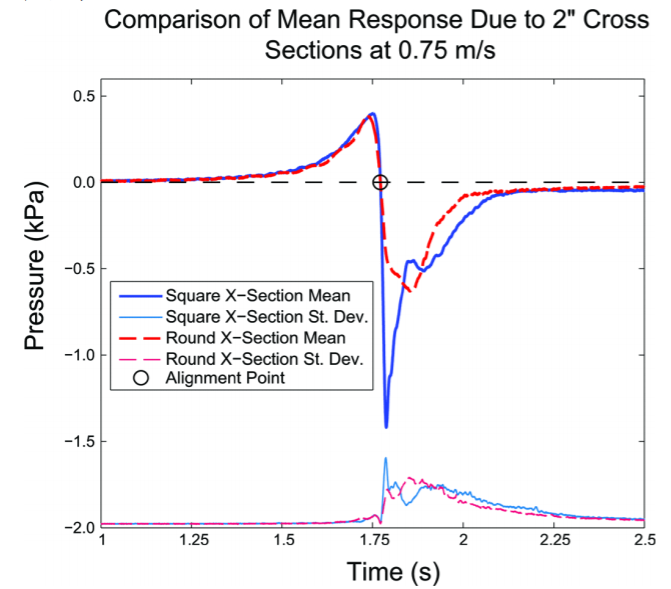
\includegraphics[width=0.50\columnwidth]{figures/Fernandez Results.png}
\end{center}
\caption{Average pressure response for square and circular cylinders, with the standard deviation offset by -2.0 kPa \citep{Fernandez2011}.}
\label{fig:PW:Square vs Circular Profiles}
\end{figure}

%\subsection{Tandem Foil Simulation with Lily Pad} \label{CFD Attempts}

    %Due to the complex equations governing vortex interactions, flow calculations are often performed using computational fluid dynamics software. Lilypad is an open source CFD program developed by Dr. G Weymouth for quick, 2D flow simulations \citep{Weymouth2015}. It solves the Navier-Stokes equations and applies body boundary conditions over surfaces using the Boundary Data Immersion Method, while maintaining a Cartesian grid for calculations \citep{Weymouth2011}. \citep{Muscutt2017} simulated tandem flapping foils using Lily Pad in order to find the effective coefficients of thrust, power, and efficiency on the downstream foil for multiple phase shifts and foil spacings. The chief benefit of fast running computational software is that a plethora of trials can be run in a fraction of the time required to run a physical test, while varying the experimental parameters with a set of keystrokes. The differential pressures between any two points can be calculated in real time for each trial and produce theoretical results for comparison to a physical model.

% This method convolves the equations governing the simulation using a kernel, creating the update equation for the convoluted velocity, \(\vec{u_e}\), and the update equation for the velocity divergence, given as
% \[\vec{u_e} =\mu_0\vec{f}+(1-\mu_0)\vec{b}+\mu_1\frac{\partial}{\partial n}(\vec{f}-\vec{b})\]
% \[\vec{\nabla}\cdot\vec{u_e}=(1-\mu_0)\vec{\nabla}\cdot\vec{b}-\mu_1\frac{\partial}{\partial n}(\vec{\nabla}\cdot\vec{b})\]
% where 